\subsection{Integration stage.} 
The outputs resulting from the four software are scanned and processed to identify both significant and best-ranked associations. MultiGWAS corrects (correction method defined in the configuration file) the p-values and calculates the threshold value for each associated marker. The calculation uses the number of valid genotype calls (i.e., non-missing genotypes, phenotypes, and covariates).

% Figure several reports
\begin{figure}
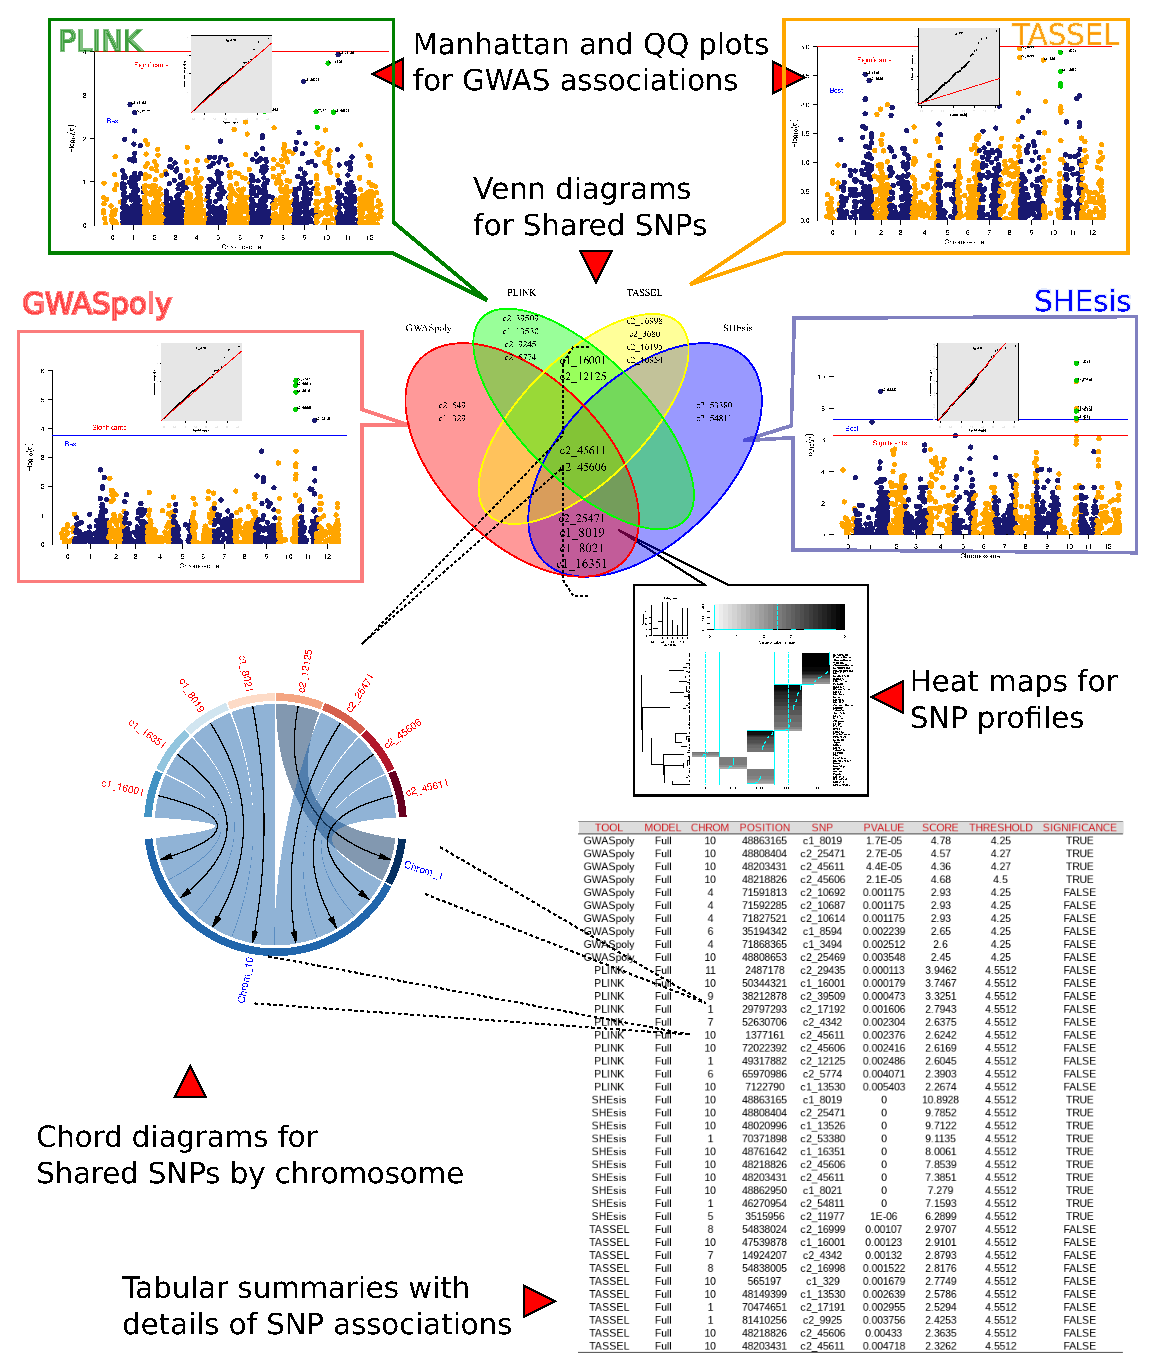
\includegraphics[width=12cm]{images/report-methodologies-all-plots}
\caption{We present several reports. For each tool, first a QQ plot that asses the resultant p-values.  Second, a Manhattan plot for each tool with two lines, blue and red, respectively, is the lower limit for the best ranked and significative SNPs. We present two Venn diagrams, one for the significative SNPs and one for N best-ranked SNPs of each tool. We show the results for GWAspoly, PLINK, TASSEL, and SHEsis in red, green, yellow, and blue, respectively. Moreover, for each SNP that is in the intersection; thus, that is predicted by more than one tool we provide SNP profile. \label{reports}}

\end{figure}

At this stage, We integrate the results to evaluate reproducible results among tools (Fig \ref{reports}). But, We still report a summary for the results of each tool:
\begin{itemize}
    \item A Quantile-Quantile (QQ) plots for the resultant p-values of each tool and the corresponding degree of inflation $\lambda$ to asses the degree of the test statistic inflation.
    \item AA Manhattan plot of each tool with two lower thresholds, one for the best-ranked SNPs, and another for the significant SNPs. 
\end{itemize}

To present the replicability, we use two sets: (1) the set of all the significative SNPs provided by each tool and (2) the set of all the best-ranked SNPs. For each set, we present a Venn diagram that shows SNPs predicted exclusively by one tool and intersections that help to identify the SNPs predicted by one, two, three, or all the tools. In addition, we provide detailed tables for the two sets.

For each SNP predicted more than once, we provide what we call the SNP profile. That is a heat diagram for a specific SNP, where each column is a genotype state AAAA, AAAB, AABB, ABBBB, BBBBB. And each row corresponds to a sample. Samples with close genotypes form together clusters. Thus to generate the clusters, we do not use the phenotype information. However, we present the phenotype information in the figure as the color. This figure visually provides information regarding genotype and phenotype information simultaneously for the whole population. We present colors as tones between white and black for color blind people. 


MultiGWAS generates a report, one document with the content previously described. Besides, there is a folder with the individual figures just in case the user needs one. In the supplementary information, we include a report and a description of the report content\textcolor{red}{(supplementary information XXX)}

%PAula: infomración suplementary con reporte completo y figuras. Y explicación del reporte

In the following section, we present the results applied to a public dataset. 
